\documentclass{beamer}
\usepackage{listings}

\title
{SIMT Branch Prediction}
\subtitle{Mitigating Stalls}
\author
{Steven Braeger \and Nick Arnold}
\institute
{
  \inst{1}%
  University of Central Florida
}
\date
{\today}

\begin{document}
\frame{\titlepage}

\begin{frame}
	\frametitle{Generic CPU Core Design}
	\begin{tabular}{c}
		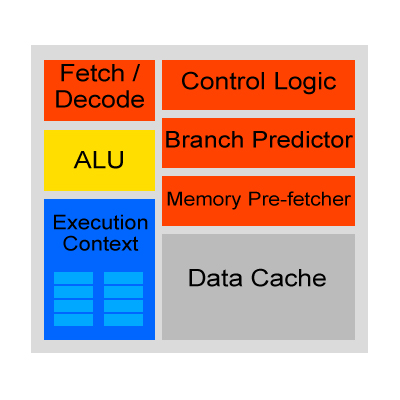
\includegraphics[width=.75\textwidth]{CPU-design.jpg}
	\end{tabular}
\end{frame}

\begin{frame}
	\frametitle{Generic CPU Core Design (cont.)}
	\begin{itemize}
		\item<1-> Regular Processor Logic
		\begin{itemize}
			\item<2-> Fetch/Decode Logic
			\item<2-> ALU for execution
			\item<2-> Execution Context (registers, etc.)
		\end{itemize}
		\item<3-> Single Thread Speedup Logic
		\begin{itemize}
			\item<4-> Control Logic
			\item<4-> Branch Predictor
			\item<4-> Memory Pre-fetcher
		\end{itemize}
		\item<5-> Data Cache
	\end{itemize}
\end{frame}

\begin{frame}
	\frametitle{Generic CPU Core Design (cont.)}
	\begin{itemize}
		\item<1-> What does this core do well?
		\begin{itemize}
			\item<2-> Single Instruction, Single Data (SISD)
			\begin{itemize}
				\item<2-> Control logic built to support this
			\end{itemize}
		\end{itemize}
		\item<3-> What does this core do poorly?
		\begin{itemize}
			\item<4-> Single Instruction, Multiple Data (SIMD)
			\item<4-> Multiple Instruction, Single Data (MISD)
			\item<4-> Miltiple Instruction, Multiple Data (MIMD)
		\end{itemize}
	\end{itemize}
\end{frame}

\begin{frame}
	\frametitle{Generic Multicore CPU Design}
	\begin{tabular}{c}
		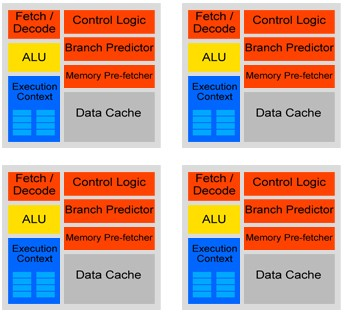
\includegraphics[width=.75\textwidth]{Multicore-CPU-design.jpg}
	\end{tabular}
\end{frame}

\begin{frame}
	\frametitle{Generic Multicore CPU Design (cont.)}
	\begin{itemize}
		\item<1-> What does this core do well?
		\begin{itemize}
			\item<2-> SISD
			\begin{itemize}
				\item<2-> Multiple independent processes
				\item<2-> Idling
			\end{itemize}
			\item<3-> MISD
			\begin{itemize}
				\item<3-> Independent instructions from one process (out of order)
			\end{itemize}
		\end{itemize}
		\item<4-> What does this core do poorly?
		\begin{itemize}
			\item<5-> SIMD
			\item<5-> MIMD
		\end{itemize}
	\end{itemize}
\end{frame}

\begin{frame}
	\frametitle{Generic GPU Core Design}
	\begin{tabular}{c}
		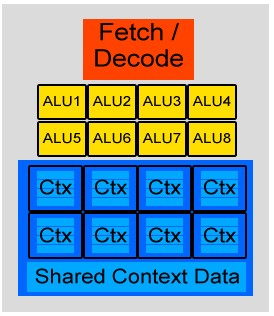
\includegraphics[width=.75\textwidth]{GPU-Design.jpg}
	\end{tabular}
\end{frame}

\begin{frame}
	\frametitle{Generic GPU Core Design (cont.)}
	\begin{itemize}
		\item<1-> What's different?
		\begin{itemize}
			\item<2-> Removed single threading speedup logic
			\item<2-> Removed data cache
			\item<2-> Added multiple execution contexts
		\end{itemize}
		\item<3-> Why do this?
		\begin{itemize}
			\item<4-> Designed for graphics processing
			\item<4-> Tailored specifically to those types of instruction streams
			\item<4-> Performing the same operations on many independent data elements
		\end{itemize}
	\end{itemize}
\end{frame}

\begin{frame}
	\frametitle{Generic GPU Core Design (cont.)}
	\begin{itemize}
		\item<1-> What does this core do well?
		\begin{itemize}
			\item<2-> SIMD
			\begin{itemize}
				\item<2-> Similar contexts assigned to GPU
				\item<2-> Core performs the same computations on all contexts
			\end{itemize}
		\end{itemize}
		\item<3-> What does this core do poorly?
		\begin{itemize}
			\item<4-> SISD
			\item<4-> MISD
			\item<4-> MIMD
		\end{itemize}
	\end{itemize}
\end{frame}

\begin{frame}
	\frametitle{Generic GPU Core Design (cont.)}
	\begin{tabular}{c}
		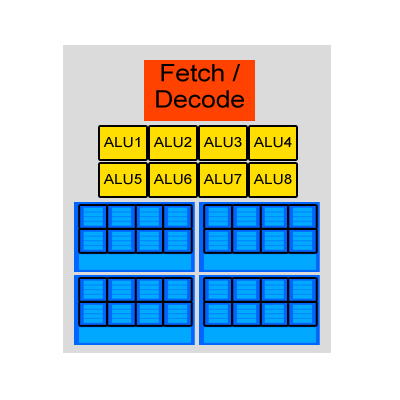
\includegraphics[width=.75\textwidth]{GPU-Design---multiple-contexts.jpg}
	\end{tabular}
\end{frame}

\begin{frame}
	\frametitle{Generic GPU Core Design (cont.)}
	\begin{itemize}
		\item<1-> GPUs can modify their context storage 
		\item<2-> Separate into various smaller contexts
		\item<3-> Try and hide stalls (more on this later)
	\end{itemize}
\end{frame}

\begin{frame}
	\frametitle{Generic Multicore GPU Design}
	\begin{tabular}{c}
		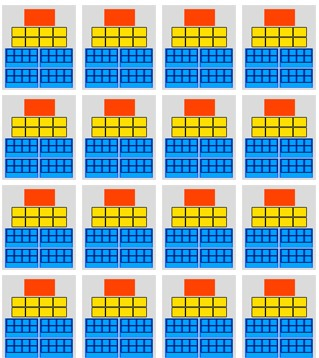
\includegraphics[width=.75\textwidth]{GPU-Design---multiple-cores.jpg}
	\end{tabular}
\end{frame}

\begin{frame}
	\frametitle{Generic Multicore GPU Design (cont.)}
	\begin{itemize}
		\item<1-> What does this core do well?
		\begin{itemize}
			\item<2-> SIMD
			\begin{itemize}
				\item<2-> All cores assigned same instruction stream
			\end{itemize}
			\item<3-> MIMD
			\begin{itemize}
				\item<3-> Multiple independent tasks (vertices, fragments, etc.)
			\end{itemize}
		\end{itemize}
		\item<4-> What does this core do poorly?
		\begin{itemize}
			\item<5-> SISD
			\item<5-> MISD
		\end{itemize}
	\end{itemize}
\end{frame}

\begin{frame}
	\frametitle{GPU Context Interleaving}
	\begin{tabular}{c}
		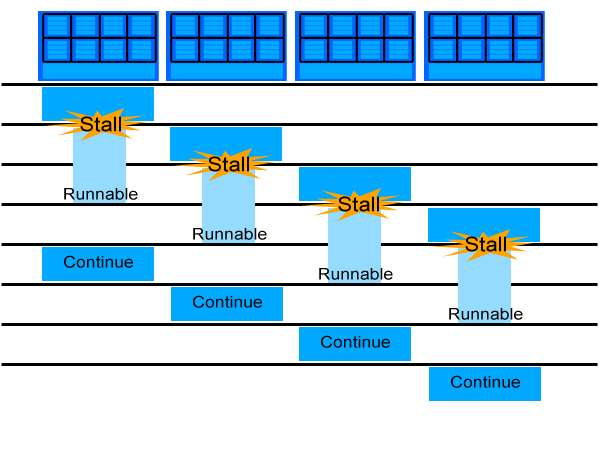
\includegraphics[width=.75\textwidth]{GPU-context-interleaving.jpg}
	\end{tabular}
\end{frame}

\begin{frame}
	\frametitle{GPU Context Interleaving (cont.)}
	\begin{itemize}
		\item<1-> GPU is always utilizing ALUs optimally, even though contexts are waiting
		\item<2-> If wait time exceeds certain amount, the GPU must stall
	\end{itemize}
\end{frame}

\begin{frame}
	\frametitle{GPU Context Interleaving (cont.)}
	\begin{tabular}{c}
		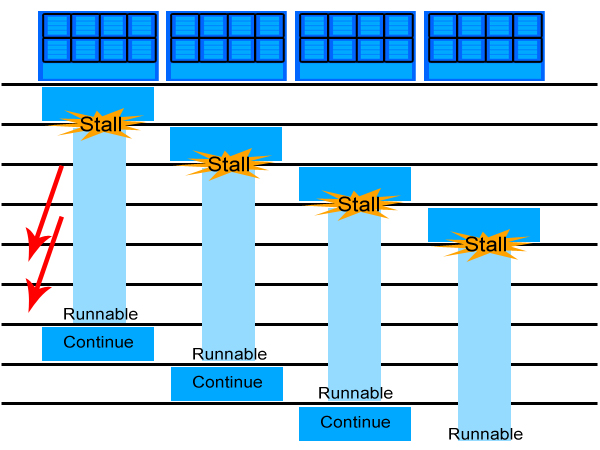
\includegraphics[width=.75\textwidth]{GPU-context-interleaving-2.jpg}
	\end{tabular}
	\begin{itemize}
		\item<1-> Red arrows indicate idle cycles due to stalling for 1st context group's branch
		\item<2-> What if we could avoid this?
	\end{itemize}
\end{frame}

\begin{frame}
	\frametitle{GPU Programs}
	\begin{itemize}
		\item<1-> GPUs bundle several contexts together into context groups
		\item<2-> Collection of all contexts belonging to one GPU core is a 'warp'
		\item<3-> All contexts within a warp will be subjected to the same instruction stream
		\begin{itemize}
			\item<3-> Processed context group by context group
			\item<3-> High degree of spatial locality
		\end{itemize}
		\item<4-> Take advantage of information discovered by the first context group 
	\end{itemize}
\end{frame}

\begin{frame}
	\frametitle{Branch Prediction on CPU}
	\begin{itemize}
		\item<1-> On CPUs, each core has one execution context and one branch prediction table
		\item<2-> Each context handles its own predictions
		\begin{itemize}
			\item<2-> No assistance from other threads 
			\item<2-> No way to guarantee what the other threads are doing
		\end{itemize}
		\item<3-> On GPUs, each core has multiple execution contexts
		\begin{itemize}
			\item<3-> All contexts assigned to that core are performing the same operations
			\item<3-> Couldn't we use this information to assist other contexts?
		\end{itemize}
	\end{itemize}
\end{frame}

\begin{frame}[fragile]
	\frametitle{Branch Prediction Example}
	\begin{itemize}
		\item<1-> Matrix Vector Multiply
		\item<2-> Parallel work ID stop in parallel
		\item<3->
	\begin{lstlisting}[language=C,basicstyle=\footnotesize,frame=single,tabsize=4,title=GemV.cl]
__kernel gemv(double * y, double * A, double * x)
{
    int rowout = cl_thread_id(0);  // index
    y[rowout] = 0.0;
    for(int i = 0; i < A.cols; i++)
        y[rowout] += A[rowout,i] * x[i];
}
	\end{lstlisting}
		\item<4-> Prediction fails to detect end of loop if BHT per thread.
		\item<5-> Shared BHT per warp mispredicts end of first rows but predicts the rest.
	\end{itemize}
\end{frame}

\begin{frame}
	\frametitle{Our Proposal}
	\begin{itemize}
		\item<1-> Introduce 3 GPU Branch Predictors with the following features
		\begin{itemize}
			\item<2-> One predictor is shared amongst the contexts within a GPU core
			\item<2-> One predictor is shared only amongst its context group (1 per group)
			\item<2-> One predictor is shared only amongst its context (1 per context)
		\end{itemize}
		\item<3-> Predictor table is the size of the instruction stream to avoid collisions
		\begin{itemize}
			\item<3-> Types of instruction streams that are issued to GPUs are by their nature not very long
		\end{itemize}
		\item<4-> Predictor table entries are Smith 2-bit predictors
		\item<5-> Compare prediction accuracies across these implementations
	\end{itemize}
\end{frame}

\begin{frame}
	\frametitle{Our Proposal (cont.)}
	\begin{tabular}{c}
		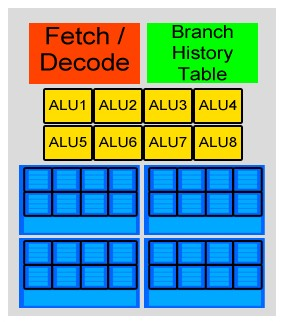
\includegraphics[width=.5\textwidth]{Our-GPU---per-core-predictor.jpg}
	\end{tabular}
\end{frame}

\begin{frame}
	\frametitle{Our Proposal (cont.)}
	\begin{tabular}{c}
		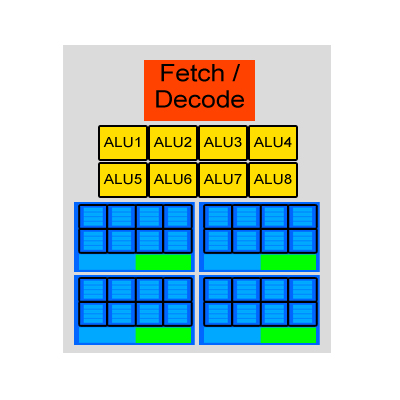
\includegraphics[width=.5\textwidth]{Our-GPU---per-context-group-predictor.jpg}
	\end{tabular}
\end{frame}

\begin{frame}
	\frametitle{Our Proposal (cont.)}
	\begin{tabular}{c}
		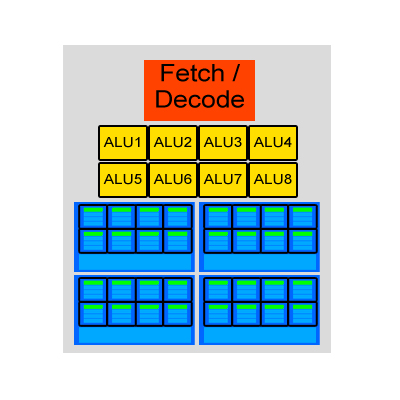
\includegraphics[width=.5\textwidth]{Our-GPU---per-element-predictor.jpg}
	\end{tabular}
	\begin{itemize}
		\item<1-> This implementation most closely resembles how a regular CPU core handles branch prediction
	\end{itemize}
\end{frame}

\begin{frame}
    \frametitle{Branch Predictor}
    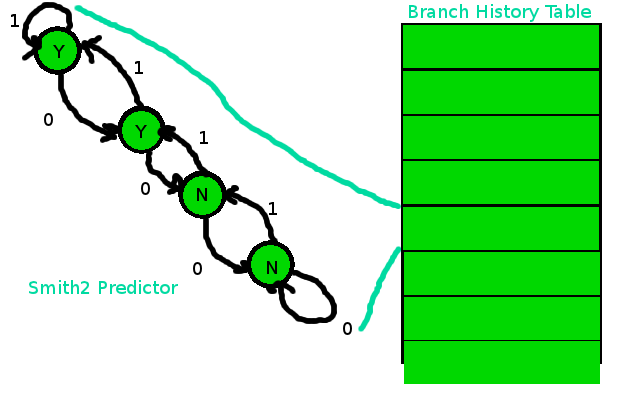
\includegraphics[height=.6\textheight]{bht.png}
    \begin{itemize}
     \item<1-> Limited Kernel Size.  Max 16k instructions.
     \item<2-> 16k BHT entries==no collisions.  4KiB of memory.
    \end{itemize}
\end{frame}


\begin{frame}
	\frametitle{Our Proposal (cont.)}
	\begin{tabular}{c}
		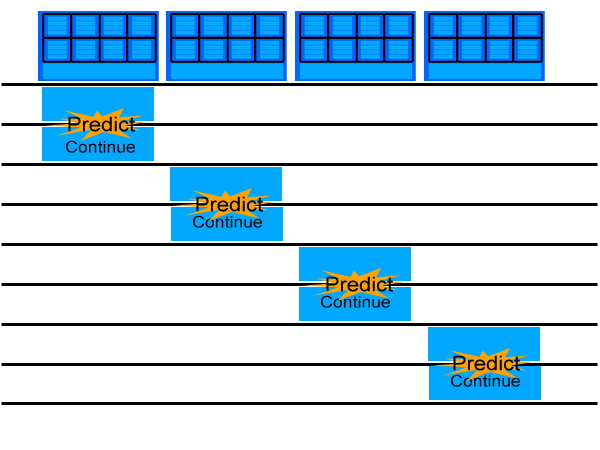
\includegraphics[width=.75\textwidth]{GPU-predict-context.jpg}
	\end{tabular}
\end{frame}

\begin{frame}
   \frametitle{Experiment}
   \begin{itemize}
    \item<1-> Must have appropriate simulator modeling SIMT architecture.
    \item<2-> SimpleScalar NOT sufficient
    \item<3-> GPGPU-Sim: Rewrite based on SimpleScalar.
    \item<4-> Simulates an NVIDIA Quadro 5800. (16k register file, 4 GB ram, 32 cores,1024 contexts)
    \item<5-> Creates libcuda.so and libOpenCL.so to intercept GPU commands from CPU program.
    \item<6-> Requires NVIDIA hardware (driver does compilation) to build benchmarks.
   \end{itemize}
\end{frame}

\begin{frame}
 \frametitle{Simulation Architecture (slide courtesy of gpgpu)}
  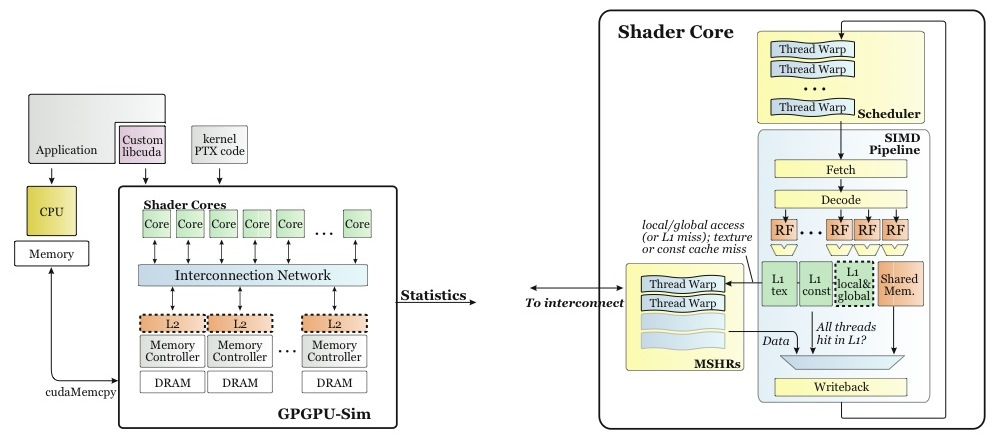
\includegraphics[width=.9\textwidth]{uarch.jpg}

\end{frame}

\begin{frame}
 \frametitle{Benchmarks (ISPASS09)}
 \begin{itemize}
  \item<1-> Subset of ISPASS09 CUDA benchmarks
  \item<2-> Some benchmarks failed
  \item<3-> Run for 4 days
  \item<4-> CPU component failed to meet dependencies
  \item<5-> CUDA Architecture unsupported (double/single)
  \item<6-> No branching!  (AES)
 \end{itemize}
\end{frame}

\begin{frame}
 \frametitle{ISPASS09 Benchmarks (cont.)}
\begin{itemize}
 \item<1-> \emph{NQU} Solve the NQUEENS problem
 \item<2-> \emph{NN} Classify images with a neural net
  \item<3-> \emph{RAY} Raytrace a scene
\item<4-> \emph{BFS} Breadth-First Search a graph.
\end{itemize}
\end{frame}

\begin{frame}
\frametitle{Results}
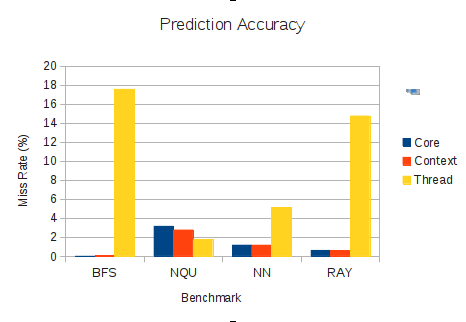
\includegraphics[width=.9\textwidth]{data.png}
\end{frame}

\begin{frame}
 \frametitle{Results (cont.)}
\begin{itemize}
 \item<1-> Significant improvement over per-thread predictor
 \item<2-> NQUEENS failed...DP solution mispredicts parallel neighbors?
\end{itemize}

\end{frame}

\begin{frame}
 \frametitle{Any Questions?}
\begin{itemize}
 \item<1-> Question: What information is available to a GPU for branch prediction that is not available for a CPU?
 \item<2-> Answer: The branch history from parallel threads in a warp or core.
\end{itemize}

\end{frame}


\begin{frame}
	\frametitle{Sources}
	\begin{itemize}
		\item Kayvon Fatahalian's SIGGRAPH 2009 Talk on How Shader Cores Work (referenced several of his diagrams)
		\item GPGPU Simulator (http://www.ece.ubc.ca/~aamodt/gpgpu-sim/)
	\end{itemize}
\end{frame}






\end{document}

